\chapter{Introduction}
\label{chap:Introduction}

\begin{quote}\small
\emph{``There are only two kinds of programming languages: \\ those people always bitch about and those nobody uses.''} \\ \hspace*{\fill}---Bjarne Stroustrup
\end{quote}
These coding notes are a short introduction to scientific programming, combined with a list of best practices.
Programming is an art; it takes time to become experienced, but these guidelines will help you to avoid common mistakes.
Follow them! They were born out of years of experience, and will save you and your instructors a lot of time.
You will be spending most of your time thinking about your algorithms and debugging your code, not actually writing it.
Writing clean code, following best practices, and not trying to be overly clever will make your life a lot easier.

Choosing a programming language is about picking the right tool for the job.
In the case of ICCP, that means Fortran.
We won't force you to use a particular language, but for most of the programs you'll write, dynamic languages such as MATLAB or Python are too slow, while C, \Cplusplus, and Java lack the built-in numerical facilities\footnote{It's called Fortran---FORmula TRANslation---for a reason!} (with Java also being slow).
Fortran is over half a century old---it first appeared in 1957---and can be a bit quirky, but for better or worse, it's still the industry standard when it comes to scientific computing.
Besides, modern Fortran---the most recent standard updates appeared in 2003 and 2008---is not nearly the monstrosity it used to be; it's actually a quite pleasant language for computational physics.
Even if you already have some experience with another language, take it from us that both you and your code will be faster if you use Fortran for ICCP.
If you want to continue in computational physics you'll encounter it sooner or later anyway (think LAPACK), and ICCP is the perfect time to learn.

These notes are by no means a Fortran reference.
High-quality documentation can be easily found online.
Good starting points are \url{http://fortran90.org} and \url{http://en.wikipedia.org/wiki/Fortran_language_features}.
The \emph{Intel Fortran Compiler Language Reference} is freely available (Google it).
We also recommend \emph{Modern Fortran Explained} by Metcalf, Reid and Cohen, or \emph{Fortran 95/2003 for Scientists \& Engineers} by Chapman.

Finally, you can find an up-to-date version of all the examples shown here (as well as useful helper modules and visualizations) at \url{https://Github.com/cglosser/libICCP}.
See the \nameref{chap:Revision control} chapter for details on cloning the code from Github.

\newpage
\null
\vfill
\begin{center}
  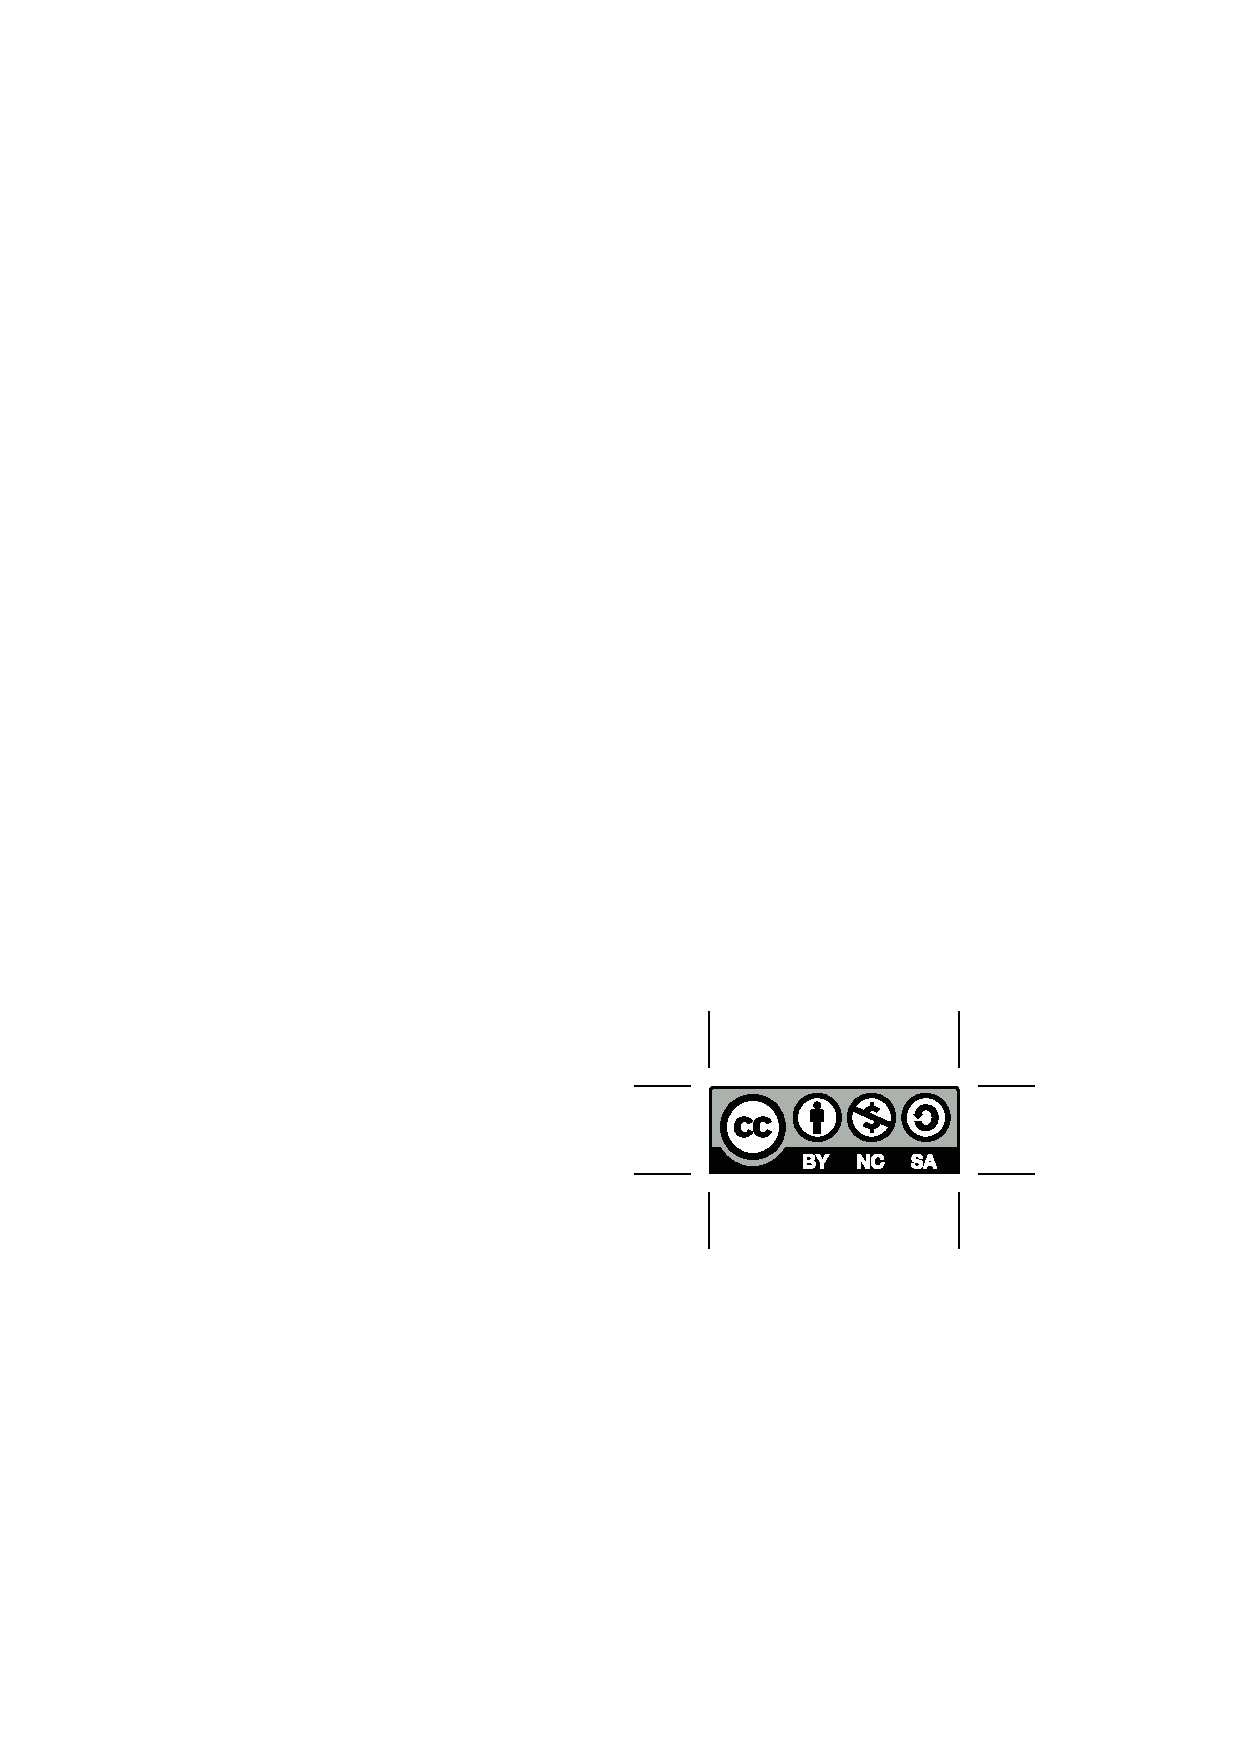
\includegraphics[width=0.15\textwidth]{figures/by-nc-sa}
\end{center}
This work---including its figures and \LaTeX\, source---is licensed under the
Creative Commons Attribution-NonCommercial-ShareAlike 4.0 International
License. To view a copy of this license, visit
\url{http://creativecommons.org/licenses/by-nc-sa/4.0/deed.en_US}.
